\documentclass[11pt]{article}
\usepackage{graphicx}
\usepackage{float}
\usepackage{amsmath}
\usepackage{listings}
\graphicspath{ {./} }
\setcounter{secnumdepth}{0}

\begin{document}
\begin{titlepage}
   \begin{center}
       \vspace*{1cm}
       \textbf{\Huge Numerical Methods} \\
       \vspace{2.0cm}
       \huge{ProjectAssignment C: Ordinary differential equations} \\
       \vspace{.7cm}
       \huge{\today} \\
       \vspace{3.0cm}
       \vspace{0.4cm}
       Krzysztof Watras\\
       \vspace{ 0.2cm }
       \small{ Tutor's name: Jakub Wagner } \\
       \vspace{2 cm}   
       \small{Computer Science} \\  
       \vspace{0.2cm}       
       \small{Warsaw University of Technology,\\
       Faculty of Electronics and Technology} \\
       \vspace{2cm}
       \small{I declare that this piece of work, which is the basis for
       recognition of achieving learning outcomes in the Numerical Methods
       course, was completed on my own. Krzysztof Watras} \\
   \end{center}
\end{titlepage} 
\tableofcontents

\newpage
\section{Introduction}
In the task provided the system of equations is the following. 
\begin{equation}
    \begin{cases}
        \displaystyle\frac{dx(t)}{dt} &= p_1x(t) - p_2x(t)y(t) \\
        \displaystyle\frac{dy(t)}{dt} &= p_3x(t)y(t) - p_4y(t) \\
    \end{cases}
\end{equation}
For $t\in[0,1],p_1=14,p_2=0.11,p_3=0.04,p_4=10,x(0)=530,y(0)=30$.\\
After substitution:
\begin{equation}
    \begin{cases}
        \displaystyle\frac{dx(t)}{dt} &= 14 x(t) - 0.11 x(t)y(t) \\
        \displaystyle\frac{dy(t)}{dt} &= 0.04 x(t)y(t) - 10 y(t) \\
    \end{cases}
\end{equation}
For $t\in [0,1]$, and $x(0) = 530, y(0) = 30$.
In MATLAB the code for it can take following form:
\lstinputlisting[language=MATLAB]{equation_given.m}

Here, we build a function that accepts the 2 element vector called $y$, and a
time span (here it is a domain) called $t$. Name $y$ can be a bit confusing because it holds
information on both $x$ and $y$ functions, but it is a standard procedure to call it that,
and it stems from the fact that $y$ is just a vector of functions instead of "usual" $y=f(x)$
format.

Here, I decided to assign label "Population" to Y axis and "Prey", "Predator"
to values of $x$ and $y$ functions because Lotka-Volterra equations are often
introduced in a context of change in population sizes depending on a current
state of the system. Very basically: if number of predators is low, number of
prey increases. But as number of prey increases number of predators rises as
well. Therefore, number of prey will fall over time, leading to decrease in the
number of predators. It serves as a good intuition as to what exactly we can 
try to solve with an ODE, or even what it actually means to solve an ODE.

\newpage
\section{Using MATLAB ode45 builtin function}
MATLAB already has a function that solves ODEs numerically, and it is called
`ode45`. It follows format as below:
\begin{lstlisting}[language=MATLAB]
    ode45(function_handle, domain, initial condition)
\end{lstlisting}

Therefore, we can use it to solve and then plot the results as seen in code below:
\lstinputlisting[language=MATLAB]{sol1.m}

This code forms graph visible on Figure~\ref{fig:ode45reference}
\begin{figure}[ht!]
    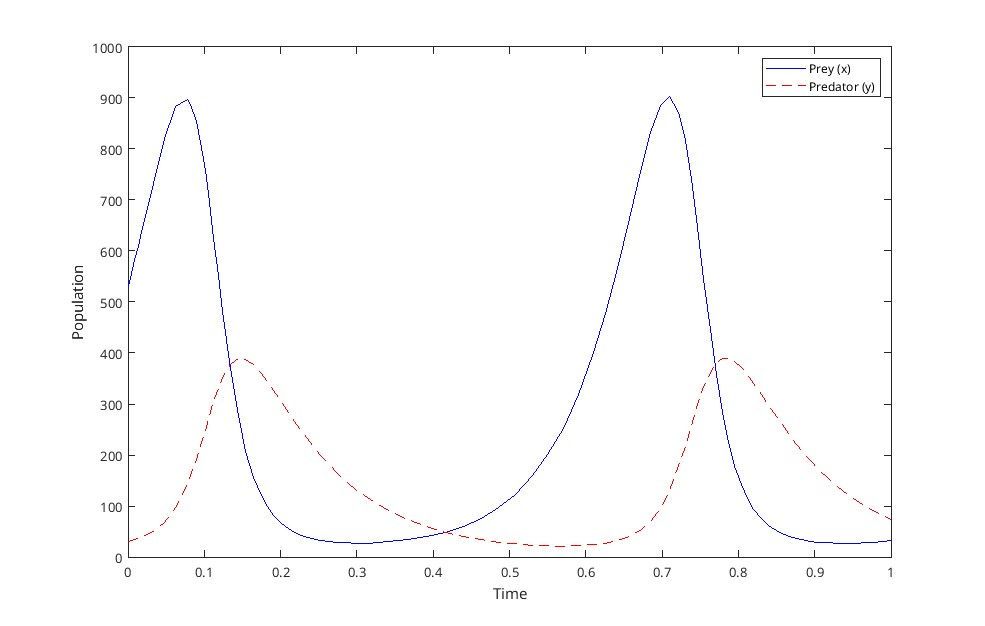
\includegraphics[width=\textwidth]{ode45reference.jpg}
    \caption{Solution obtained using ode45 function}
    \label{fig:ode45reference}
\end{figure}

\newpage
\section{Explicit Euler method}
Considering a general first order differential equation
\begin{equation}
    \frac{dy}{dx} = f(t,y); y(t_0) = y_0,
    \label{eq:general_first_order_eq}
\end{equation}
that we want to solve on some interval $[t_0, t_n]$. 
Our goal is to approximate solution of $y(x)$ at each $t$ in domain.
Since $y(t_0)$ is given the first value we need to estimate is $y(t_1)$.
Using Taylor's Theorem, we can write 
$$y(t_1) = y(t_0) + y'(t_0)(t_1 - t_0) + \frac{y'(c)}{2}(t_1-t_0),$$
where $c \in (t_0,t_1)$. Knowing Equation~\ref{eq:general_first_order_eq}, we have
$$y(t_1) = y(t_0) + f(t_0, y(t_0))(t_1-t_0) + \frac{y'(c)}{2}(t_1-t_0),$$

Let us call $\Delta t = (t_1 - t_0)$. When $\Delta t$ is small enough, the term $\frac{y'(c)}{2}(t_1-t_0)$ is small enough to be treated as an error term.
This way we obtain:
\begin{equation}
    y(t_1) \approx y(t_0) + f(t_0, y(t_0))\cdot \Delta t
    \label{eq:euler_formula_particular}
\end{equation}

It follows trivially that this is true for any step of the algorithm therefore we can write
\begin{equation}
    y(t_{k+1}) \approx y(t_k) + f(t_k, y(t_k))\cdot \Delta t
    \label{eq:euler_formula_general}
\end{equation}
where $k = 1,2,\dots,n-1$, and $\Delta t$ can be described more
generally as $\Delta t = (t_{k+1} - t_k) = \frac{t_n-t_0}{n}$ \\
Finally, we get 
\begin{equation}
    y_{k+1} \approx y_k + f(t_k, y_k)\cdot \Delta t
    \label{eq:euler_formula_final}
\end{equation}

This leads us to write it in MATLAB code:
\lstinputlisting[language=MATLAB]{euler_explicit.m}

Some formulas above were inspired by brilliant resource linked in reference section $[2]$. 
One can also find a good explenation on different methods not covered in this report.

\section{Implicit Euler method}
In this method, we do the same thing but this time we do it implicily, ie. we
start with some guess and then, iterate to find proper solution.

This manifests in following code:
\lstinputlisting[language=MATLAB]{euler_implicit.m}

\section{Comparison of results for different methods}
Before numerical comparison let us see how all methods look on common graph.

\begin{figure}[ht!]
    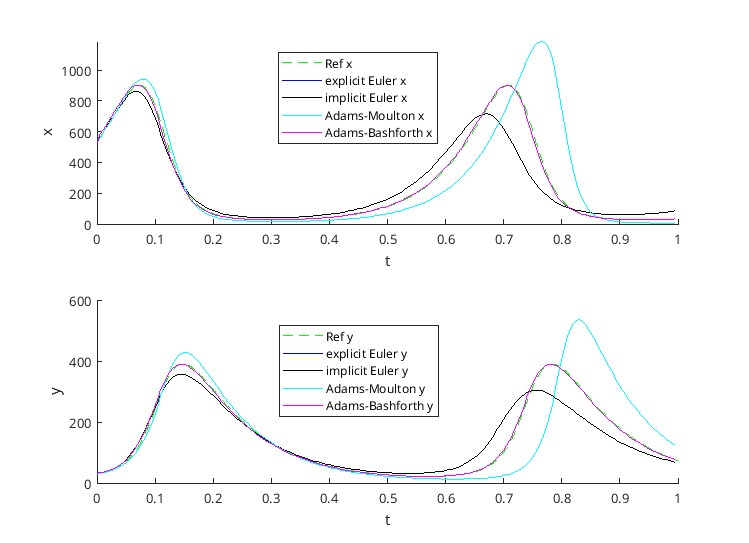
\includegraphics[width=\textwidth]{combined.jpg}
    \caption{Combined graph for all solutions}
    \label{fig:combined_methods}
\end{figure}

As we see on the Figure~\ref{fig:combined_methods}, 
explicit Euler method although simple and intuitive, can lead to
large errors resulting from compounding. 
The implicit version however yielded much better results. What appears to be
the best method so far is Adams-Bashforth method. Its shape resembles the
reference one very closely, almost identically.

After this initial analysis, let us focus on actual numerical values of the errors found.
When we run code from file $sol3.m$ we can see output that equals one in the Table 1.

\begin{table}[H]
    \caption{Total aggregated error for each method compared to ode45 reference}
    \label{tab:aggregated_error}
    \begin{center}
        \begin{tabular}{l|l}
            Method & Aggregated error \\
            \hline
            Explicit Euler & 0.4559 \\
            Implicit Euler & 0.1748 \\
            Adams-Moulton & 0.2136 \\
            Adams-Bashforth & 0.0015 \\
        \end{tabular}
    \end{center}
\end{table}

\subsection{Change in aggregated error depending on size of step of integration}
\begin{figure}[ht!]
    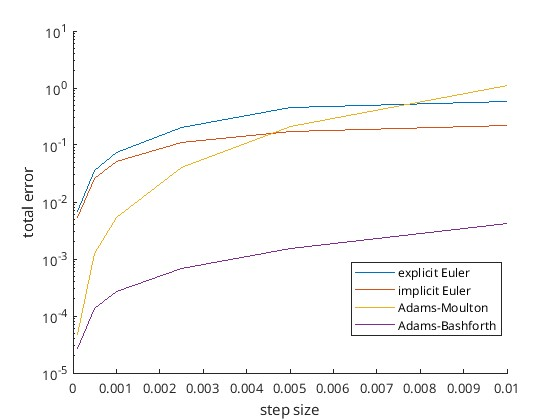
\includegraphics[width=\textwidth]{./errorOnStepSize.jpg}
    \caption{Aggregated error depending on the iteration step}
    \label{fig:errorOnStepSize}
\end{figure}

As one can see in Figure 3, the bigger the step size the bigger the total error.
This is unsurprising, as the "true" solution would be obtained for continous case.
Here it would be impractical (due to calculation time as well as cumulative
numerical errors) but can be approached via small step size.
The best method for all iteration sizes is Adams-Bashforth method. And the
worst is explicit Euler method. What is interesting, the Adams-Moulton and
implicit Euler methods swap places as step size changed. This means that
results in previous task are valid but should not form our intuition on general
performance equations of the algorithms.

\section{Finding minimum p vector values for given set of points}
In task 5 we are given a set of points that represent a certain state of function in time.
Our task is to find such values of p such that they can be approached with our set of equations.

As a minimizing function we are given:
$$J(\textbf{p}) = \sum_{n=1}^N (\hat{x}_n(\textbf{p}) - \tilde{x}_n)^2 +
\sum_{n=1}^N (\hat{y}_n(\textbf{p}) - \tilde{y}_n)^2$$

We are to use \textbf{fminsearch} to find those values.

Minimized values of \textbf{p} are:

\begin{table}[H]
    \caption{Minimized values of \textbf{p}}
    \label{tab:aggregated_error}
    \begin{center}
        \begin{tabular}{l|l}
            $p_n$ & value \\
            \hline
            $p_1$ & 6.8162 \\
            $p_2$ & 0.1028 \\
            $p_3$ & 0.0380 \\
            $p_4$ & 16.1954 \\
        \end{tabular}
    \end{center}
\end{table}

And a graph that visualizes the difference:
\begin{figure}[H]
    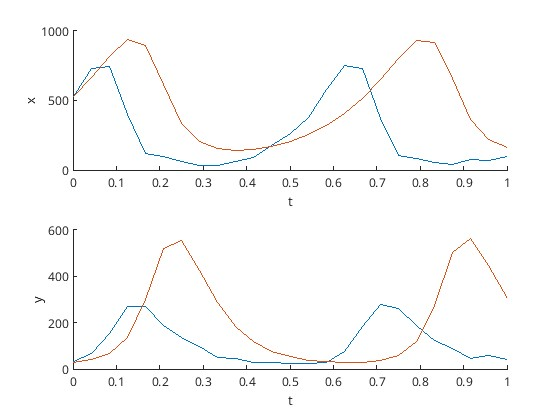
\includegraphics[width=\textwidth]{./minimized_graphs.jpg}
    \caption{Minimized graph vs the original data points}
    \label{fig:minimized_graphs}
\end{figure}

As one can see in Figure~\ref{fig:minimized_graphs}, the minimized value of the
ODE does not cover the original values (but resemble the general shape to some
extent).

\newpage
\section{Summary and conclusions}
It comes as a no surprise that different methods come with unique pros and cons.
Some have greater precision, some are more intuitive, some are easier to
implement than others. Overall, Adams-Bashforth method proved to be most
accurate for this ODE. 

Despite not solving the equation perfectly (most likely as a result of an error
of mine) the \textbf{fminsearch} can prove to be useful if one wants to find
the parameters that describe data the best.

Another takeaway from this task is to make the code solving the equations as general as one can get.
My current solution has code duplication that makes the code more confusing that it needs to be.
This can be easily improved had it not been for a terrible time management that plagued this project. 
Crucially: one should never attempt solving a set of ODEs a day before deadline!
This one vital part caused quite a lot of mistakes that could have been easily avoided with more time spent on the project.

Overall, this task showed the importance of knowing different methods for solving ODEs as that can lead to better results in the solution.

\newpage
\section{References}
{[1]} R. Z. Morawski: Numerical methods (ENUME) – \emph{6. Solving ordinary
differential equations}, Warsaw University of Technology, Faculty of
Electronics and Information Technology \\
{[2]} https://www.math.tamu.edu/~phoward/m401/matode.pdf

\newpage
\section{Appendix: Listing of the developed programs}
\subsection{Source code for Task 1}
\lstinputlisting[language=MATLAB]{sol1.m}
\newpage
\subsection{Source code for Task 2}
\lstinputlisting[language=MATLAB]{sol2.m}
\newpage
\subsection{Source code for Task 3}
\lstinputlisting[language=MATLAB]{sol3.m}
\newpage
\subsection{Source code for Task 4}
\lstinputlisting[language=MATLAB]{sol4.m}
\newpage
\subsection{Source code for Task 5}
\lstinputlisting[language=MATLAB]{sol5.m}
\newpage
\subsection{Source code for J optimizer}
\lstinputlisting[language=MATLAB]{J.m}
\newpage
\subsection{Source code for explicit Euler method}
\lstinputlisting[language=MATLAB]{./euler_explicit.m}
\newpage
\subsection{Source code for implicit Euler method}
\lstinputlisting[language=MATLAB]{./euler_implicit.m}
\newpage
\subsection{Source code for Adams-Moulton method}
\lstinputlisting[language=MATLAB]{./Adams_Moulton.m}
\newpage
\subsection{Source code for Adams-Bashforth method}
\lstinputlisting[language=MATLAB]{./Adams_Bashforth.m}
\end{document}

